\section{Deutsch-Jozsa Problem}
Deutsch-Jozsa is an ``upgraded'' version of Deutsch's problem. The problem set up is the following. \\
Given $f: \binset^n \to \binset$, we are \impt{promised} that it is either constant ($\forall \mathbf{x} \in \binset^n, f(\mathbf{x}) = b$) or balanced (half of $\mathbf{x} \in \binset^n, f(\mathbf{x}) = 0$, the other half gives $1$). We want to decide which case we are in. \\
The quantum circuit that solves this problem is the following:
\begin{center}
    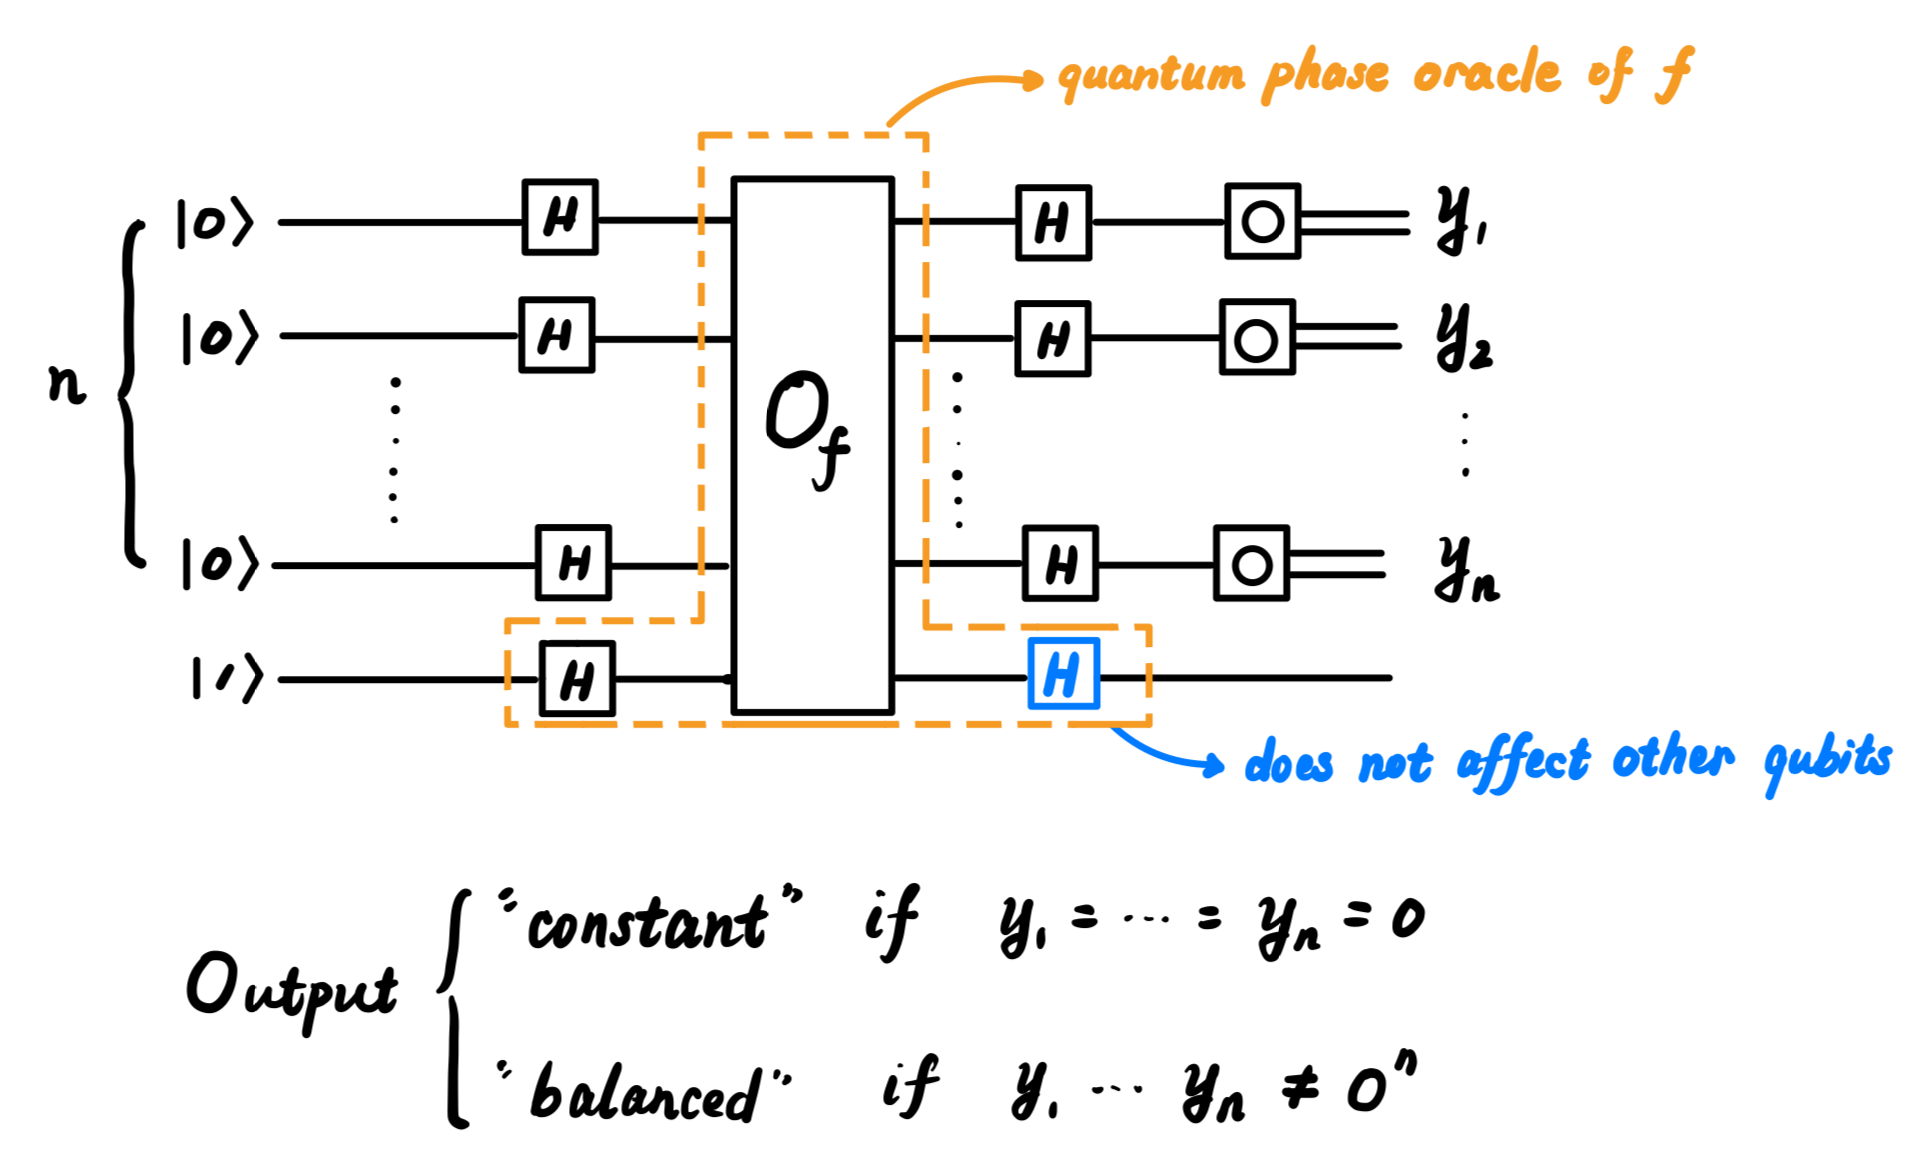
\includegraphics[scale = 0.2]{6/deutsch-jozsa.png}
\end{center}
The \impt{quantum phase oracle} of $f$ mentioned in this circuit is given by:
$$\opuni_f: \mathbf{x}\ket{b} \mapsto (-1)^{b \cdot f(\mathbf{x})}\ket{\mathbf{x}}\ket{b}$$
One useful lemma for analysis is that
\begin{lemma}
    Given $b \in \binset$, we have
    $$H\ket{b} = \frac{1}{\sqrt{2}}(\ket{0} + (-1)^b\ket{1}$$
    This extends to
    $$H^n \ket{\mathbf{x}} = \frac{1}{\sqrt{2^n}} \Sumi{\mathbf{y} \in \binset^n} (-1)^{\mathbf{x} \cdot \mathbf{y}}\ket{\mathbf{y}}$$
    where
    $$\mathbf{x} \cdot \mathbf{y} = \Sum{i = 1}{n} x_i \cdot y_i$$
\end{lemma}
Another useful mathematical trick is that
$$(-1)^{1 \oplus b} = -(-1)^b$$
where $b \in \binset$. \\
The speedup of this quantum circuit is obvious. If we use a classical query model, we need $2^{n-1} + 1$ times to be certain. In this model, we need one quantum query to be certain. \\
However, this \impt{does not} mean we have an unconditional provable exponential quantum speedup, becuase once we instantiate $f$ as a classical circuit, there may be more efficient ways of solving the D-J problem classically, by analyzing the circuit and just querying it. \\
Being only able to query the circuit for $f$ is the essential simplifying assumption of the query model.


\newpage